\section{Solutions Proposées}
%les solutions proposées dans la literature sont faites en amont, nous pouvons clasifier ces solutions en 2 categories
\subsection{Première Catégorie}
\begin{frame}{title sub section}
\begin{wrapfigure}{r}{0.3\textwidth}
	\vspace{-35pt}
	\begin{center}
		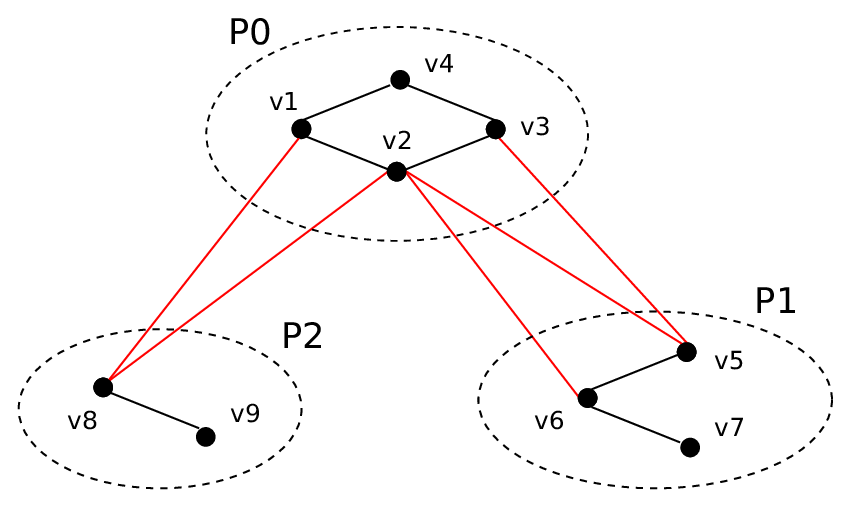
\includegraphics[width=0.2\textwidth]{resources/partitions}
	\end{center}
	\vspace{-35pt}
	\end{wrapfigure}
       Les approches de cette catégorie aboutissent à un meilleur équilibrage de charge entre les différentes machines.
       
       
		\begin{columns}
      		\begin{column}{0.3\textwidth}
   				\only<2->
      			{
	      			\begin{figure}
	      				\centering
	      				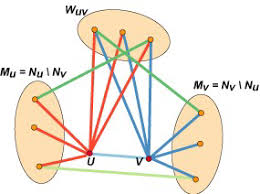
\includegraphics[width=\linewidth]{resources/transitions}
	      			\end{figure}   
      			}   			
      		\end{column}
      	
	      	\begin{column}{0.7\textwidth}
      			\only<3->
	      		{
	      		\begin{block}{Problèmes}
	      			\begin{itemize}
	      			\only<4->
	      			{	
	      				\item Distribution statique.% la distribution reste intacte tout au long du model cheking
	      			}
      				\only<5->
      				{
	      				\item Nombre de Transitons externes minimum implique -t-il réduction du taux de communication?% pourai entrainer un nombre elever de communications	 
	      			}
      				\only<6->
      				{     				
	      				\item La puissance des machines non exploitée.% il peut y avoir des machines qui effetue peut de calcule alors que les autres un nombre elevé de calcul
	      			}
	      			\only<7->
	      			{
	      				\item Temps de réponse non raisonnable.
	      			}
	      			\end{itemize}
	      		\end{block}
      		  }
	      	\end{column}
      	\end{columns}
     
\end{frame}

\subsection{Deuxième Catégorie}
\begin{frame}{title sub section}
\begin{wrapfigure}{r}{0.3\textwidth}
	\vspace{-20pt}
	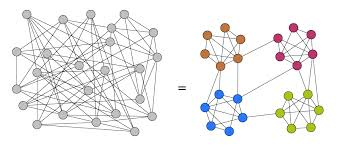
\includegraphics[width=0.3\textwidth]{resources/transition}
	\vspace{-20pt}
\end{wrapfigure}
La philosophie de cette catégorie vise à minimiser les transitions externes avec un bon équilibrage de charge entre les différentes machines.
 
 \only<2->
 {
		%\item Distribution statique.% la distribution reste intacte tout au long du model cheking
		\begin{columns}
			\begin{column}{0.3\textwidth}
				\centering
				\begin{figure}
					\begin{tikzpicture}		

						\node [inner sep=-10pt,visible on=<1-4>]{
							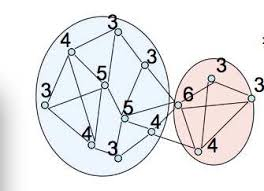
\includegraphics[height=1.2in,width=\columnwidth,trim={0 0 0 0},clip]{resources/bequilibre}
						};              
					
					\node [inner sep=-10pt,visible on=<5->]
					{
						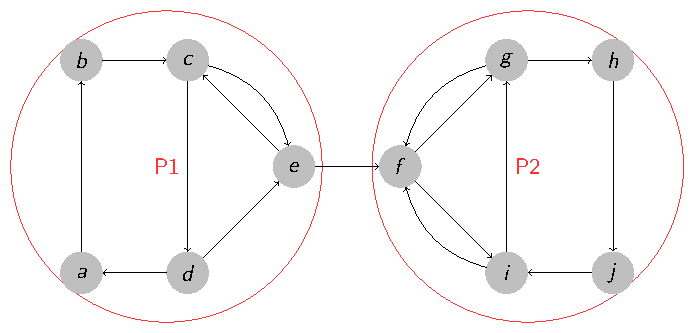
\includegraphics[height=1.2in,width=\columnwidth,trim={0 0 0 0},clip]{resources/contre_exemple}
					}; 
					\node[inner sep=-10pt,visible on=<6->](expressions) at (-1.3,-1.8) {AG\(f\)};             
			
					\end{tikzpicture}
				\end{figure}
			\end{column}
		
         \begin{column}{0.7\textwidth}
         	
         	\begin{block}{Problèmes}
         		\begin{itemize}
         		\item Distribution statique.% la distribution reste intacte tout au long du model cheking
         		\item L'équilibrage peut être dégradé.% pourai entrainer un nombre elever de communications
         		\item La puissance des machines non exploitée.% il peut y avoir des machines qui effetue peut de calcule alors que les autres un nombre elevé de calcul         		
         	 \end{itemize}
           \end{block}
         \end{column}
		\end{columns}
}
 \vspace{0.5cm}
 \only<4->
 {
	\textbf{ Minimisation des transitions externes \color{red} $\stackrel{?}{\Rightarrow}$ Temps de réponse minimisé}.  
}
\end{frame}

\subsection{Solution en aval}
\begin{frame}
	\centering
	\vspace{2.2cm}       
	\Huge 
	\textbf{Solution en aval}
	%chercher a surcharger une machine faira qu'augmenter le temps de la verification
\end{frame}

\begin{frame}{title sub section}
  
  
  
\begin{center}
	\begin{columns}
		\begin{column}{\textwidth}
			\begin{figure}				
				\begin{tikzpicture}		
				\only<1-1>
				{
					\node [inner sep=-10pt]
					{
						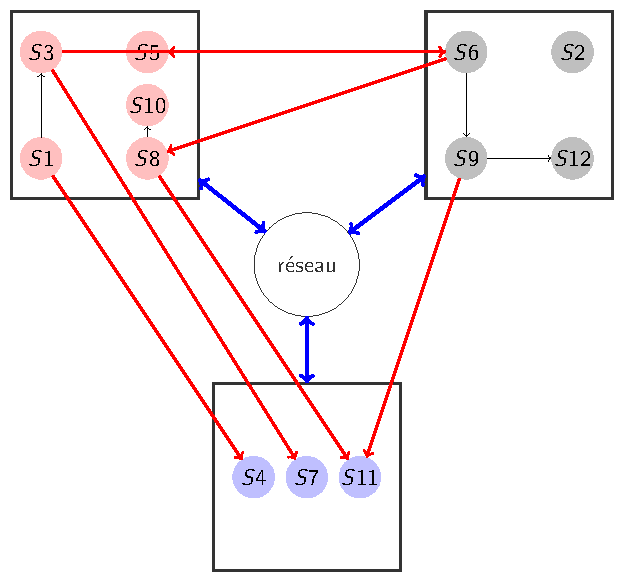
\includegraphics[height=1.8in,width=0.7\columnwidth,trim={0 0 0 0},clip]{resources/benstira/0001}
					};              
				}
			\only<2-2>
			{
				\node [inner sep=-10pt]
				{
					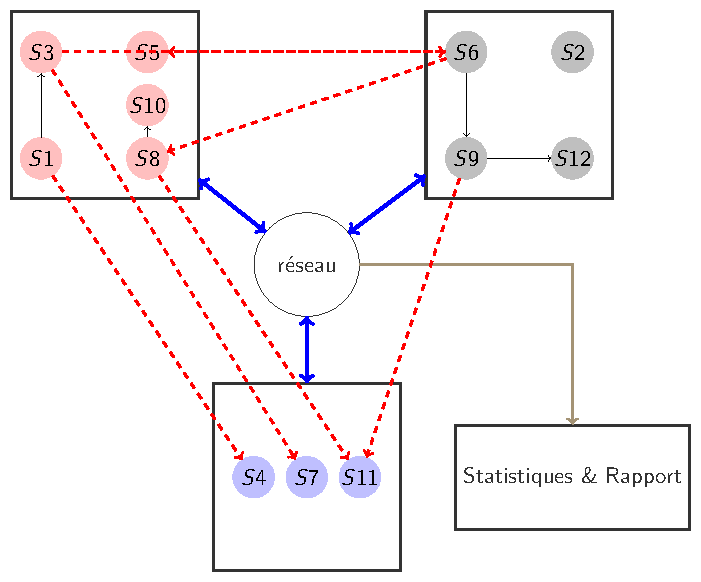
\includegraphics[height=1.8in,width=0.7\columnwidth,trim={0 0 0 0},clip]{resources/benstira/0002}
				};              
			}
			\only<3-3>
			{
				\node [inner sep=-10pt]
				{
					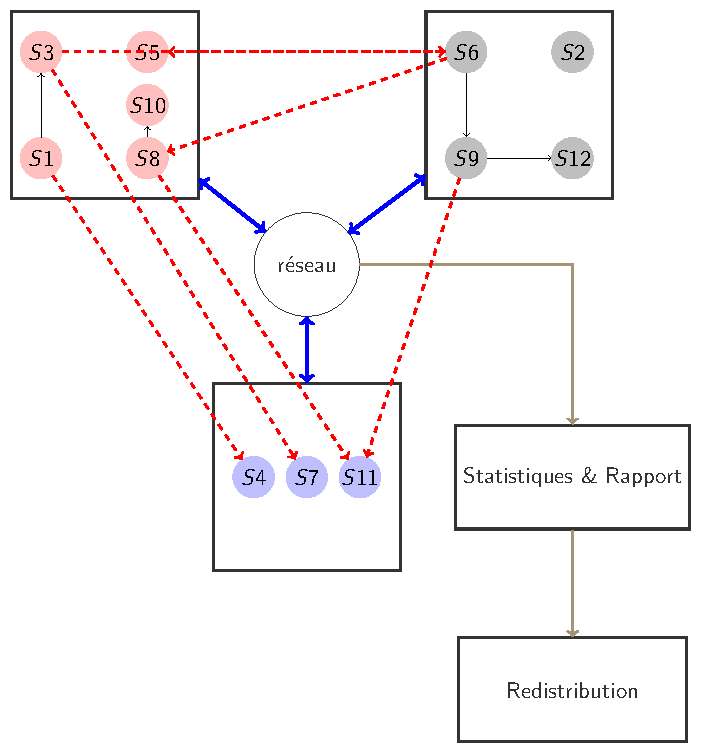
\includegraphics[height=2in,width=0.7\columnwidth,trim={0 0 0 0},clip]{resources/benstira/0003}
				};              
			}
			\only<4-4>
			{
				\node [inner sep=-10pt]
				{
					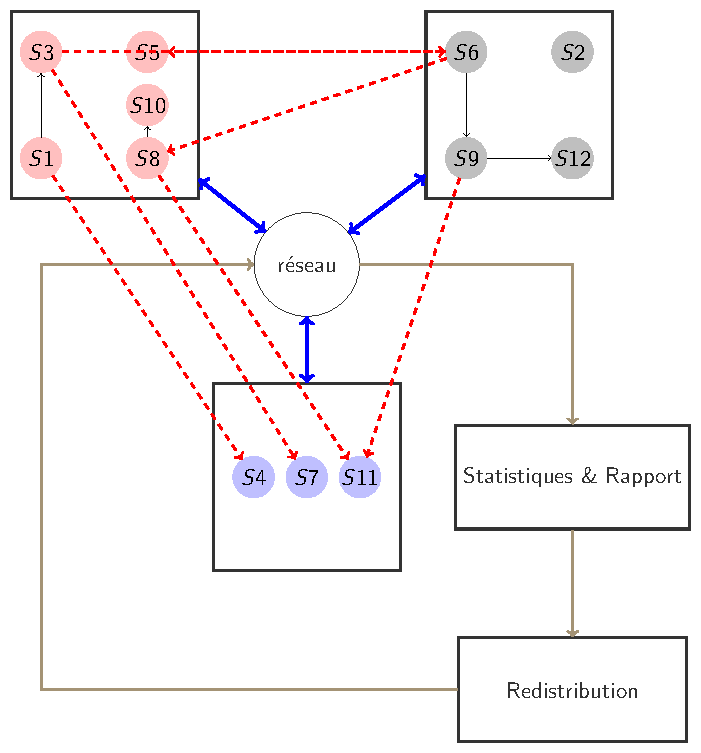
\includegraphics[height=2in,width=0.7\columnwidth,trim={0 0 0 0},clip]{resources/benstira/0004}
				};              
			}		
				\end{tikzpicture}				
				
			\end{figure}
		\end{column}
	\end{columns}
\end{center}
\end{frame}

\begin{frame}
	\centering
	\vspace{2.2cm}       
	\Huge 
	\textbf{Critiques}	
\end{frame}

\begin{frame}{tite subsection}
\vspace{-10pt}
\begin{block}{Critiques}
	\vspace{-15pt}
	\begin{columns}
		\begin{column}{\textwidth}
			\begin{itemize}
				\item Minimisations des transitions externes.
				\item Duplications et Migrations basées sur les transitions.
				\item Certains machines peuvent être surchargées de calcul ou de stockage.
				\item Duplication de certains états est sans intérêt.% sinon le model checking sera faux
			\end{itemize}
		\end{column}
	\end{columns}
\only<2->
{
	\begin{columns}
		\begin{column}{0.3\textwidth}
			\centering
			\begin{figure}				
				\begin{tikzpicture}		
					\only<2-4>
					{
						\node [inner sep=-10pt]
						{
							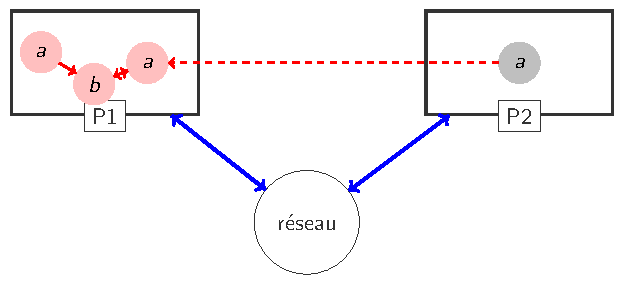
\includegraphics[height=1.2in,width=\columnwidth,trim={0 0 0 0},clip]{resources/benstira/critque1}
						};              
					}
					
					\node [inner sep=-10pt,visible on=<4-4>]
					{
						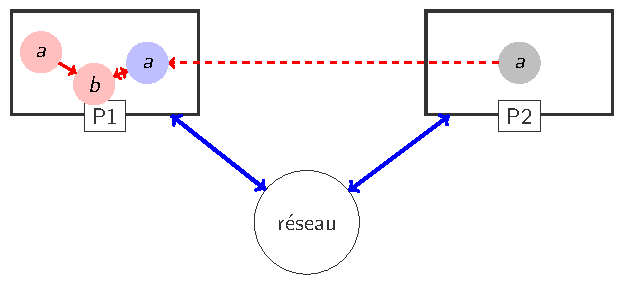
\includegraphics[height=1.2in,width=\columnwidth,trim={0 0 0 0},clip]{resources/benstira/critque2}
					};  
				
					\node [inner sep=-10pt,visible on=<5-5>]
					{
						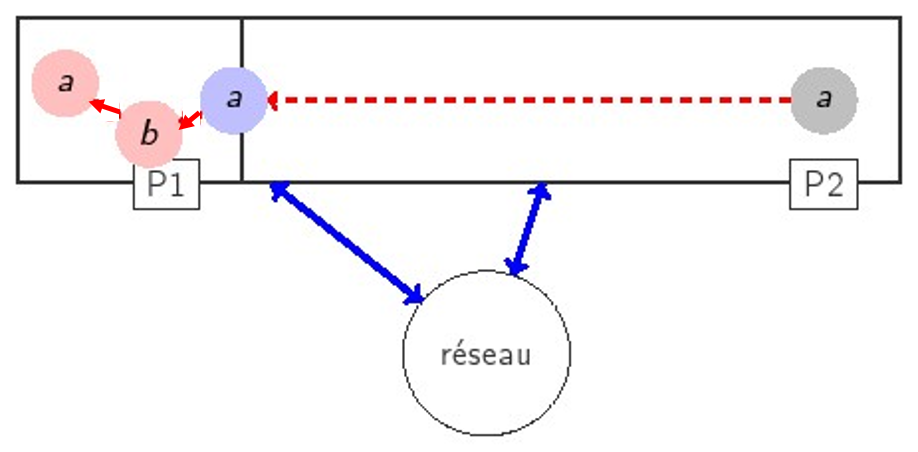
\includegraphics[height=1.2in,width=\columnwidth,trim={0 0 0 0},clip]{resources/benstira/critque3}
					};                
			% question est ce que le temps est amelioré? si oui le model checking sera fausse, sinon la duplication n'a rien servi
				\end{tikzpicture}				
			\end{figure}
		\end{column}
		\begin{column}{0.7\textwidth}
			\begin{itemize}
				\item AG(a)
				\only<3->
				{
				\item Si 0.45 < L/$N_t$ ≤ 0.75, alors dupliqué \color{red}{\tiny \citep{BENSETIRA2017}}.
			}
			\end{itemize}
		\end{column}
	\end{columns}
}
\end{block}
\end{frame}